\documentclass[journal]{IEEEtran}
\usepackage[utf8]{inputenc}
\usepackage[T1]{fontenc}
\usepackage[spanish,english]{babel}
\usepackage{graphicx}
\usepackage{amsmath}
\usepackage{booktabs}
\usepackage{array}
\usepackage{cite}
\usepackage{url}
\usepackage{xurl}
\usepackage[hidelinks]{hyperref}
\usepackage{microtype}
\usepackage{balance}
\interdisplaylinepenalty=2500
\graphicspath{{figures/}}
\hyphenation{time-tabling curri-cu-lum Lecture-Kick}

\title{Planificación de Horarios Universitarios: revisión del estado del arte y estudio de reproducibilidad en CB-CTT}
\author{Jorge Martin La Peña, Alejandro Moris Lara y Jose Miguel Villacorta Arteaga%
\thanks{Máster Universitario en Aprendizaje Automático y Datos Masivos, Universidad Politécnica de Madrid.}}

\begin{document}
\maketitle


\selectlanguage{spanish}

\begin{center}\begin{minipage}{\columnwidth}\small\textbf{Resumen---} La planificación de horarios universitarios constituye un problema de optimización combinatoria en el que deben asignarse sesiones docentes a periodos y aulas satisfaciendo restricciones obligatorias y minimizando criterios de calidad. Este trabajo presenta una revisión del estado del arte del Curriculum-Based Course Timetabling Problem (CB-CTT) durante 2015--2026, complementada con un estudio experimental de reproducibilidad sobre la formulación UD2 de ITC-2007. El corpus analizado contiene 25 estudios primarios y cubre métodos exactos y declarativos, metaheurísticas, enfoques híbridos, hiperheurísticas y técnicas de selección y configuración automática de algoritmos. En este corpus, ITC-2007 aparece explícitamente en el 64\% de los estudios y el aprendizaje automático se utiliza principalmente como apoyo para seleccionar, caracterizar o configurar métodos de optimización. Para evaluar la reproducibilidad se ejecutó BHC-KSA con el vecindario LectureKick de Ceschia et al. sobre 19 instancias no redundantes de ITC-2007 UD2, con tres semillas por instancia y 57 ejecuciones en total. Todas produjeron horarios factibles sin violaciones duras. La reproducción se contrasta funcionalmente con el protocolo del artículo de 2026 y, de forma separada, su competitividad se mide frente a los mejores valores conocidos de la literatura: el mejor coste reproducido igualó ese best-known en dos instancias. Las diferencias se interpretan considerando el menor número de repeticiones y el cambio de entorno computacional. En el corpus analizado, los datos de benchmark son mayoritariamente públicos, pero el código y las configuraciones completas son mucho menos frecuentes.\par\vspace{0.35em}\textbf{Palabras clave---} planificación de horarios universitarios, CB-CTT, ITC-2007, metaheurísticas, optimización combinatoria, reproducibilidad, LectureKick.\end{minipage}\end{center}

\selectlanguage{english}

\begin{abstract}
University course timetabling is a combinatorial optimization problem in which teaching activities must be assigned to time periods and rooms while satisfying mandatory constraints and minimizing quality penalties. This paper presents a state-of-the-art review of the Curriculum-Based Course Timetabling Problem (CB-CTT) covering 2015--2026, complemented by an experimental reproducibility study using the ITC-2007 UD2 formulation. The analyzed corpus contains 25 primary studies covering exact and declarative methods, metaheuristics, hybrid approaches, hyper-heuristics, and algorithm selection and automatic configuration techniques. Within this corpus, ITC-2007 is explicitly used in 64\% of the studies, while machine learning is mainly employed to support algorithm selection, instance characterization, and solver configuration. Reproducibility was evaluated using BHC-KSA with the LectureKick neighborhood proposed by Ceschia et al. on 19 non-redundant ITC-2007 UD2 instances, with three random seeds per instance and 57 runs in total. All runs produced feasible timetables with no hard-constraint violations. The reproduction is assessed functionally against the 2026 paper protocol, while competitiveness is evaluated separately against literature best-known values: the best reproduced cost matched that best-known value on two instances. Differences are interpreted in light of the reduced number of repetitions and the different computational environment. In the analyzed corpus, benchmark data are mostly public, whereas source code and complete experimental configurations are far less common.
\end{abstract}

\begin{IEEEkeywords}
university course timetabling, CB-CTT, ITC-2007, metaheuristics, combinatorial optimization, reproducibility, LectureKick.
\end{IEEEkeywords}

\selectlanguage{spanish}

\section{Problema de investigación}

La planificación de horarios universitarios exige coordinar sesiones docentes, profesorado y aulas. La dificultad consiste en encontrar una asignación compatible con los recursos disponibles y con criterios de calidad docente. Este trabajo estudia el Curriculum-Based Course Timetabling (CB-CTT), en particular la formulación UD2 utilizada en el tercer track de ITC-2007, y combina una revisión crítica de métodos y benchmarks con la reproducción de un artefacto reciente de búsqueda local.


En CB-CTT se asigna un periodo y un aula a cada sesión de una semana lectiva. Un currículo agrupa asignaturas que comparten alumnado; por ello, sus sesiones no deben coincidir. Las restricciones duras exigen programar todas las sesiones en periodos distintos para cada asignatura, impedir coincidencias de aula, profesor o currículo y respetar las indisponibilidades. Un horario es factible cuando satisface todas ellas \cite{ref1}.


La calidad de los horarios factibles se evalúa mediante la suma ponderada de cuatro penalizaciones. En UD2, la capacidad del aula es una restricción blanda: superar sus plazas aumenta el coste, pero no invalida por sí solo el horario \cite{ref1}.


\begin{table}[!b]
\caption{Penalizaciones de ITC-2007 Track 3. Fuente: \cite{ref1}.}
\label{tab:penalizaciones}
\centering
\footnotesize
\begin{tabular}{p{0.29\columnwidth} p{0.58\columnwidth}}
\toprule
\textbf{Criterio} & \textbf{Penalización en UD2}\\
\midrule
Capacidad & 1 punto por estudiante sin plaza y sesión.\\
Días mínimos de docencia & 5 puntos por día faltante respecto al mínimo de la asignatura.\\
Compactación del currículo & 2 puntos por sesión aislada y currículo, sin sesión adyacente del mismo currículo ese día.\\
Estabilidad del aula & 1 punto por aula distinta adicional utilizada por una asignatura.\\
\bottomrule
\end{tabular}
\end{table}

\section{Objetivos y preguntas de investigación}

El objetivo general es caracterizar la evolución reciente de los métodos para CB-CTT, analizar el papel de sus benchmarks y tendencias de adaptación, y evaluar hasta qué punto puede reproducirse un resultado reciente mediante artefactos públicos. El estudio mantiene ITC-2007 UD2 como referencia experimental principal e ITC-2019 como contexto para discutir la evolución hacia formulaciones universitarias más ricas.


Se plantean cuatro preguntas de investigación: RQ1, qué enfoques algorítmicos se han utilizado para CB-CTT entre 2015 y 2026 y cómo han evolucionado; RQ2, cómo han evolucionado los benchmarks, qué escalas y características cubren y qué papel conserva ITC-2007; RQ3, qué tendencias recientes aparecen en hibridación, hiperheurísticas, selección de algoritmos, configuración automática y aprendizaje automático; y RQ4, hasta qué punto pueden reproducirse resultados recientes usando implementaciones, configuraciones y benchmarks públicos.


\section{Búsqueda y selección bibliográfica}

La búsqueda se cerró el 4 de octubre de 2026 y utilizó como ventana principal 2015--2026, conservando trabajos anteriores únicamente cuando eran fundacionales para el problema, el benchmark o una línea metodológica. Se consultaron páginas editoriales, repositorios institucionales y de autores, recursos oficiales de benchmarks y literatura localizada mediante seguimiento de referencias. Como anclas para el snowballing se utilizaron las revisiones de Bettinelli et al. \cite{ref3}, Ceschia et al. \cite{ref2} y Gu et al. \cite{ref4}. Entre las consultas ejecutadas figuraron «"curriculum based course timetabling"», «"CB-CTT"», combinaciones con «exact methods», «constraint programming», «algorithm selection», «hyper-heuristic», «hybrid», «adaptive» y consultas específicas sobre ITC-2019.


El cribado aplicó criterios explícitos. Se incluyeron estudios de 2015--2026 que abordaran CB-CTT o una extensión directamente relacionada, propusieran o evaluaran un método computacional, reportaran resultados o análisis de benchmark, utilizaran datos identificables y dispusieran de suficiente información académica. Se excluyeron trabajos centrados únicamente en exámenes o enseñanza escolar, duplicados, documentos sin evidencia suficiente y publicaciones anteriores a 2015 que no fueran fundacionales. De 40 candidatos se incluyeron 25 estudios primarios: 21 de CB-CTT central y 4 extensiones explícitas; 13 documentos se conservaron solo como contexto y 2 se excluyeron.


Para cada estudio primario se extrajeron año, familia y método, benchmark o datos, escala, métricas, comparadores, resultado principal, disponibilidad de datos y código, evidencia de reproducibilidad y cobertura de RQ. Esta matriz sustenta los recuentos y figuras cuantitativas de la Sección~\ref{subsec:reviewquant}. La matriz completa de cribado y extracción, con DOI/URL y decisión de inclusión, se conserva como material suplementario de la entrega (Matriz\_Maestra\_CB-CTT\_Screening\_2015-2026\_v5\_Data\_Extraction.xlsx); por tanto, los porcentajes reportados no proceden de un recuento bibliográfico implícito.


\section{Benchmarks de referencia}

ITC-2007 Track 3 proporciona 21 instancias procedentes de la Universidad de Udine, publicadas en tres conjuntos de siete. Constituye el benchmark principal de este trabajo por disponer de una definición común de factibilidad y coste \cite{ref1}. La revisión de Ceschia et al. \cite{ref2} depura esta colección: excluye comp11, cuyo óptimo cero alcanzan consistentemente los métodos competitivos, y comp15, equivalente a comp03 bajo UD2. La propuesta adopta así 19 instancias de evaluación; esta selección no modifica el tamaño original del benchmark.


ITC-2019 responde a un modelo más amplio. Integra la asignación de clases a horarios y aulas con la distribución de estudiantes entre grupos, conocida como student sectioning. Permite configuraciones de teoría, prácticas o laboratorios, patrones de días y semanas y restricciones de distribución. La descripción de sus organizadores documenta 30 instancias competitivas y seis de prueba, procedentes de diez universidades \cite{ref5}.


La función objetivo de ITC-2019 combina penalizaciones de tiempo, aula, distribución y conflictos de estudiantes, con pesos definidos en la instancia \cite{ref5}. Sus puntuaciones no son directamente comparables con el coste UD2. La diferencia central es el modelo de decisión: ITC-2007 emplea currículos predefinidos para representar conflictos, mientras que ITC-2019 incorpora la asignación de estudiantes a grupos. Por tanto, ambas denominaciones deben acompañarse de su formulación al identificar los datos utilizados en un artículo.


\section{Estado del arte}

\subsection{Métodos exactos y basados en restricciones}

\subsubsection{Programación entera y descomposición}

La programación lineal entera mixta (MIP o MILP) representa las asignaciones mediante variables binarias y expresa las restricciones como relaciones algebraicas. La búsqueda por ramificación y acotación, reforzada con cortes válidos, puede producir horarios y cotas inferiores \cite{ref3}. En minimización, un horario factible proporciona una cota superior; una cota inferior certifica un valor por debajo del cual no puede situarse el óptimo. Cuando ambas coinciden se demuestra optimalidad. Si se agota el tiempo antes de cerrar esa diferencia, la mejor solución encontrada no debe presentarse como óptima.


La estructura de la formulación influye en su rendimiento. Bagger, Kristiansen, Sørensen y Stidsen \cite{ref6} desarrollan modelos que conectan la planificación temporal y la asignación de aulas mediante flujos. Su formulación basada en flujo de coste mínimo reduce las variables enteras respecto a una formulación directa y obtiene, en sus experimentos, mejores cotas superiores medias que los otros enfoques MIP comparados. La contribución muestra que explotar la estructura del problema puede ser tan relevante como elegir el solver; no acredita una superioridad universal sobre todas las familias de algoritmos.


Bagger, Sørensen y Stidsen \cite{ref7} aplican descomposición de Dantzig-Wolfe y generación de columnas a patrones diarios. En el conjunto de 20 instancias de su estudio, mejoran las cotas inferiores de las cuatro que permanecían abiertas y reducen la brecha media de esas cuatro del 24 \% al 11 \%. Es una mejora de la estimación del óptimo, no una reducción equivalente del coste de los horarios. El procedimiento calcula cotas; el artículo no presenta un algoritmo completo de branch-and-price. Estos resultados describen la comparación publicada en 2019, no el estado actual de todas las instancias.


\subsubsection{Restricciones y modelos lógicos}

La programación por restricciones (CP) trabaja con dominios de valores y propaga restricciones para descartar asignaciones incompatibles. La satisfacibilidad proposicional (SAT) formula la factibilidad mediante cláusulas lógicas, mientras que MaxSAT parcial ponderado permite optimizar penalizaciones manteniendo cláusulas obligatorias. Asín Achá y Nieuwenhuis \cite{ref8} constituyen un antecedente de su aplicación a CB-CTT. Esta distinción entre satisfacer restricciones y optimizar el coste también es esencial al interpretar los métodos recientes.


La programación de conjuntos de respuesta (ASP) ofrece otro paradigma declarativo. Banbara et al. \cite{ref9} desarrollan teaspoon y evalúan 61 instancias bajo cinco formulaciones, es decir, 305 combinaciones. Informan de 54 mejoras de resultados previos, incluidas 16 nuevas soluciones óptimas. Estas cifras corresponden al conjunto de formulaciones y configuraciones analizado, no exclusivamente a las 21 instancias originales de ITC-2007 UD2. Su aportación es relevante tanto para expresar variantes del problema como para obtener certificados en parte de los casos.


El análisis distingue tres aportaciones diferentes: obtener un horario factible, establecer una cota inferior y certificar un óptimo. Separarlas evita interpretar una mejora de cota como si fuese necesariamente una mejora equivalente del horario producido.


\subsection{Metaheurísticas}

Una vez alcanzada la factibilidad, el espacio de soluciones sigue siendo muy amplio; por ello, una parte sustancial de la literatura de CB-CTT recurre a metaheurísticas y búsqueda local \cite{ref2}. Estas técnicas exploran vecindarios de horarios y utilizan reglas de aceptación o mecanismos de diversificación para escapar de óptimos locales.


Los primeros trabajos sobre CB-CTT combinaron movimientos de reasignación e intercambio con Hill Climbing y búsqueda tabú. En la Segunda Competición Internacional de Horarios de 2007 (Second International Timetabling Competition, ITC-2007), el método de Müller obtuvo el mejor resultado en la modalidad dedicada a este problema. Su propuesta coordina cinco tipos de movimiento con Hill Climbing, Gran Diluvio (Great Deluge) y enfriamiento simulado \cite{ref10}. Hill Climbing conserva los cambios que mejoran el horario, Great Deluge utiliza un umbral de aceptación que varía durante la búsqueda y el enfriamiento simulado permite aceptar algunos empeoramientos.


En un problema de minimización, el enfriamiento simulado acepta siempre una mejora y admite un empeoramiento de magnitud $\Delta$ con probabilidad $\exp(-\Delta/T)$. La temperatura T disminuye durante la ejecución. Al principio se aceptan más cambios desfavorables, lo que permite salir de un horario que parece bueno solo dentro de su entorno inmediato. Conforme baja la temperatura, esos cambios se vuelven menos probables y la búsqueda se concentra en reducir el coste. La Fig.~\ref{fig:sa} resume este ciclo. En el problema estudiado, cada solución nueva es un horario vecino y la decisión de aceptarlo depende del cambio en la penalización y de la temperatura.


\begin{figure}[!t]
\centering
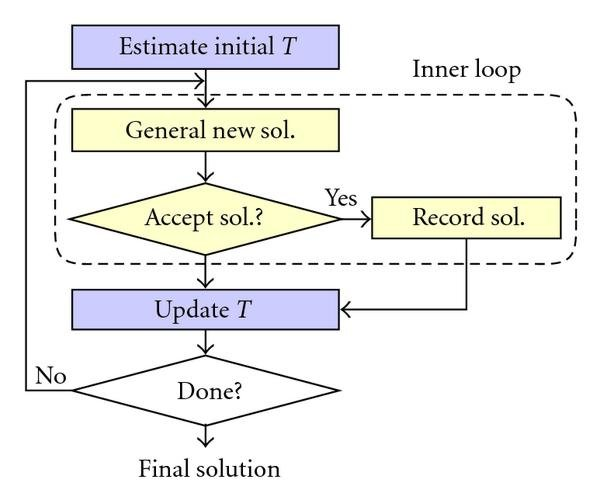
\includegraphics[width=0.92\columnwidth]{fig1.png}
\caption{Ciclo general del enfriamiento simulado. Para CB-CTT, la nueva solución corresponde a un horario vecino y la temperatura regula la aceptación de los cambios que aumentan su penalización. Reproducido de la Fig. 1 de Ababei \cite{ref11}.}
\label{fig:sa}
\end{figure}

Bellio et al. aplicaron este esquema a CB-CTT y mostraron que la temperatura inicial influye de forma directa en la calidad final \cite{ref12}. Song et al. lo ampliaron con varios tipos de movimiento y ajustaron la frecuencia con la que se seleccionaba cada uno \cite{ref13}. Cuando existen varios movimientos, la búsqueda también debe decidir cuál aplicar en cada momento. La búsqueda de vecindario variable (Variable Neighborhood Search, VNS) cambia de vecindario cuando el actual deja de producir mejoras. El descenso por vecindarios variables (Variable Neighborhood Descent, VND) sigue una secuencia fijada de búsquedas locales. Las hiperheurísticas llevan esta decisión a un nivel superior y seleccionan el movimiento de bajo nivel que se aplicará a continuación.


Otros métodos amplían la búsqueda manteniendo varios horarios a la vez. Abdullah et al. combinan una población de soluciones con un mecanismo inspirado en electromagnetismo y Great Deluge \cite{ref14}. La incorporación de componentes con funciones diferentes conduce a los métodos híbridos, cuyo uso creciente en planificación universitaria recoge la revisión de Abdipoor et al. \cite{ref15}.


\subsection{Métodos híbridos}

Los métodos híbridos combinan técnicas que intervienen en momentos distintos de la búsqueda. Un algoritmo memético, por ejemplo, genera varios horarios y aplica una búsqueda local para mejorar algunos de ellos. En una matheurística, el algoritmo retira temporalmente un conjunto de clases del horario y formula su recolocación como un problema matemático. Kiefer et al. siguen este segundo enfoque mediante una búsqueda adaptativa de gran vecindario (Adaptive Large Neighborhood Search, ALNS) \cite{ref16}. La parte adaptativa elige qué clases conviene retirar según el rendimiento reciente de cada regla y el modelo exacto vuelve a asignarlas sin alterar el resto del horario. Así se exploran cambios amplios sin perder el control sobre las restricciones.


Otra posibilidad consiste en combinar una población de horarios con una regla de aceptación propia de la búsqueda local. Abdullah et al. asignan a cada horario una fuerza calculada a partir de su penalización y emplean esa información para dirigir Great Deluge \cite{ref14}. La Fig.~\ref{fig:hybrid} muestra el mecanismo sobre horarios concretos. Las soluciones con menor penalización atraen la búsqueda, las peores la alejan y la combinación produce un nuevo horario.


\begin{figure}[!t]
\centering
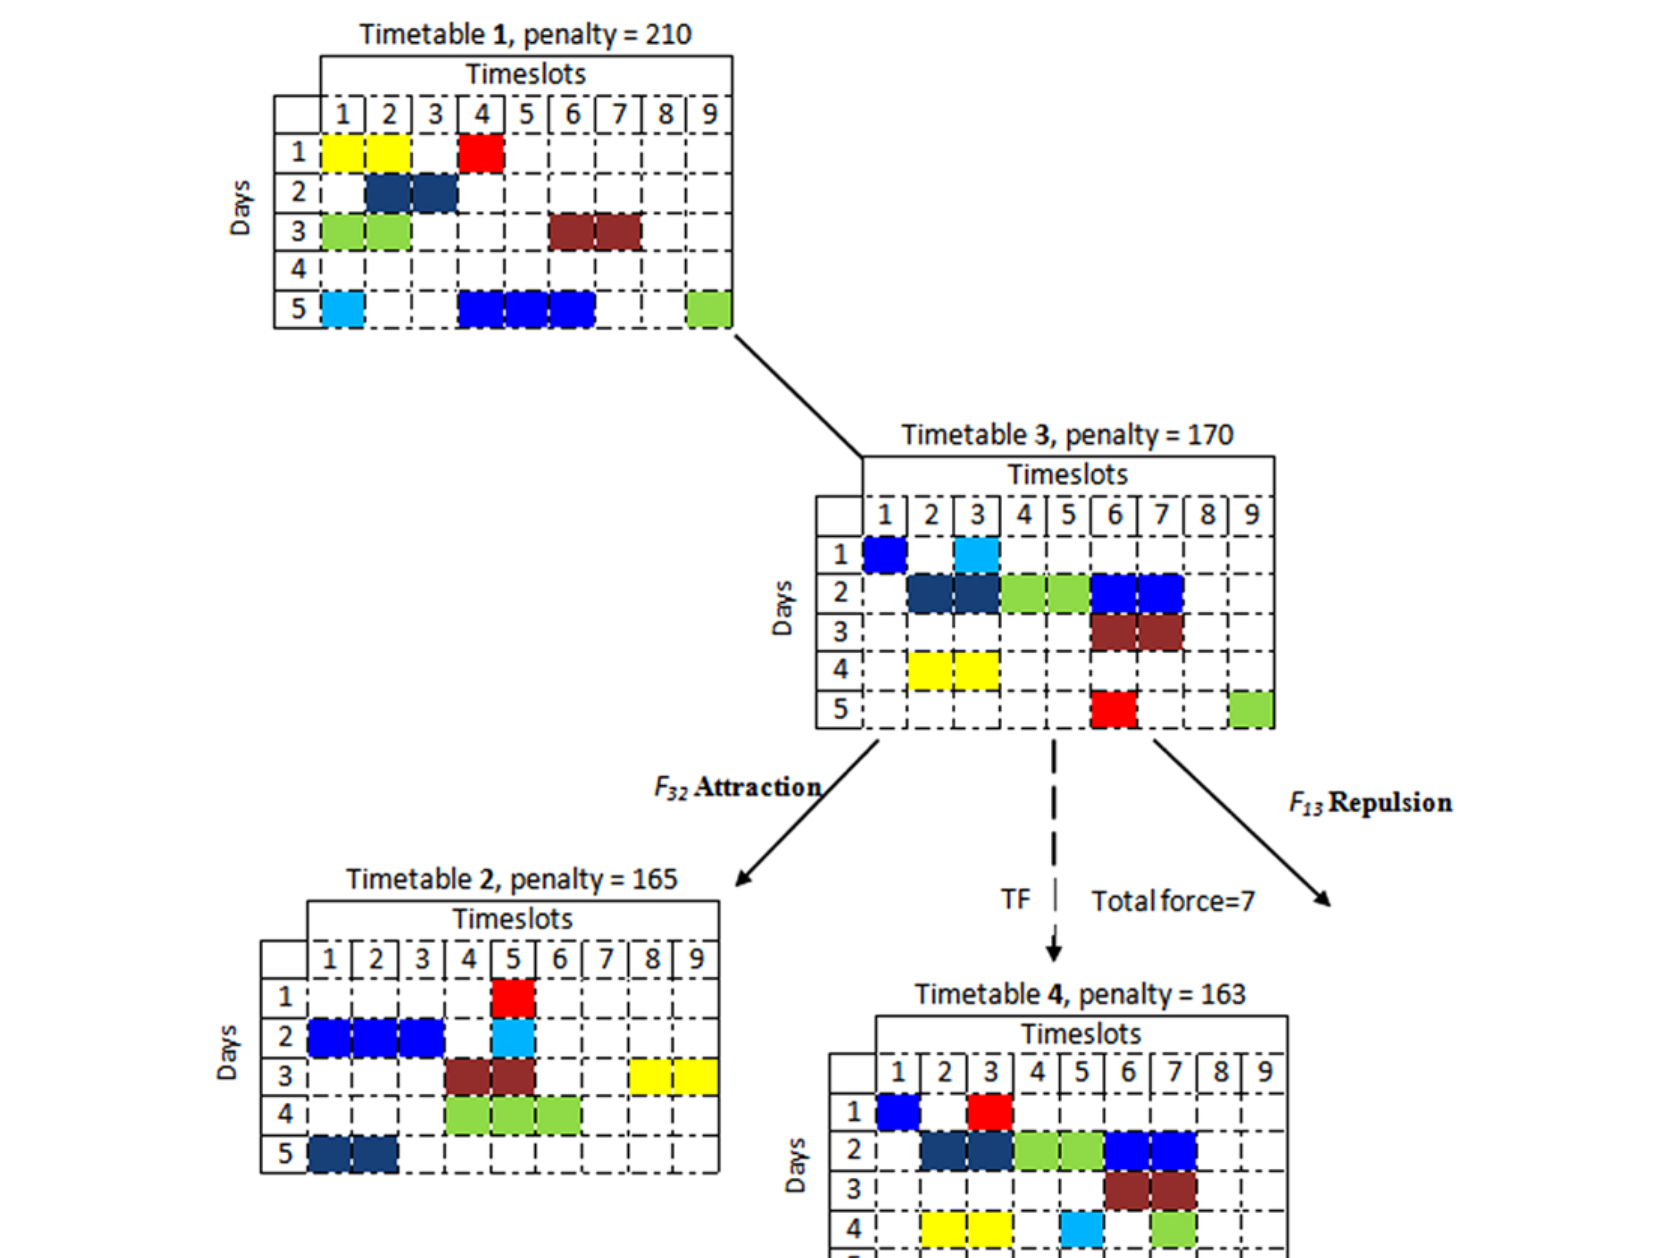
\includegraphics[width=0.98\columnwidth]{fig2.png}
\caption{Ejemplo del componente de atracción y repulsión del método híbrido de Abdullah et al. Los horarios con penalizaciones 210 y 165 modifican la búsqueda iniciada desde el horario con penalización 170, que conduce a una nueva solución con penalización 163. Reproducido de la Fig. 2 de Abdullah et al. \cite{ref14}.}
\label{fig:hybrid}
\end{figure}

\subsection{Nuevas líneas de investigación}

Una línea reciente estudia cómo adaptar el algoritmo a cada instancia antes de comenzar la búsqueda. De Coster et al. describen cada problema mediante 256 características y entrenan selectores que recomiendan el algoritmo más apropiado para cada región del espacio de instancias \cite{ref17}. Este planteamiento desplaza la pregunta desde qué método es mejor en promedio hacia qué método conviene utilizar ante una estructura concreta de conflictos, aulas y disponibilidad.


Una línea reciente estudia cómo adaptar el algoritmo a cada instancia o combinar construcción exacta y mejora local. De Coster et al. describen cada problema mediante 256 características y entrenan selectores que recomiendan el algoritmo más apropiado para distintas regiones del espacio de instancias \cite{ref17}. En 2026, Nguyen combina una inicialización CP-SAT con VND y perturbación guiada por penalizaciones sobre ITC-2007 \cite{ref21}. En conjunto, estas propuestas desplazan la pregunta desde qué método es mejor en promedio hacia qué método o configuración conviene utilizar ante una estructura concreta de conflictos, aulas y disponibilidad.


En el método que se reproduce, Hill Climbing obtiene un horario factible y el enfriamiento simulado decide si acepta cada modificación. LectureKick es la regla que construye esa modificación respetando las restricciones del horario. Por eso el vecindario conecta la estrategia de aceptación con la estructura concreta de CB-CTT.


\section{El vecindario LectureKick}

LectureKick es la regla de vecindario con la que el algoritmo genera el siguiente horario. Ceschia et al. la aplican después de una inicialización mediante Hill Climbing y dentro de una fase de enfriamiento simulado \cite{ref18}. La regla reubica una o dos clases sin incumplir las restricciones obligatorias. Antes de aplicarla, el programa construye un horario factible y calcula las cuatro penalizaciones blandas del problema.


Cada clase ocupa un hueco definido por un periodo y un aula. En la nota$c_i$ón de la Fig.~\ref{fig:lecturekick}, $l_i$ identifica una clase, $c_i$ indica el curso al que pertenece esa clase y $s_i$ representa un hueco del horario. Por ejemplo, $l_2$:$c_2$ $s_i$gnifica que la segunda clase pertenece al curso $c_2$. LectureKick parte de $l_1$ $s_i$tuada en $s_1$ y propone trasladarla a $s_2$. Si el destino está $l_i$bre, basta con mover $l_1$. Cuando $s_2$ contiene otra clase $l_2$, LectureMove solo permite enviarla al hueco $l_i$berado $s_1$. LectureKick añade la po$s_i$bi$l_i$dad de colocar $l_2$ en cualquier hueco $l_i$bre $s_3$. De este modo puede alcanzar horarios que no están disponibles mediante un intercambio directo.


\begin{figure}[!t]
\centering
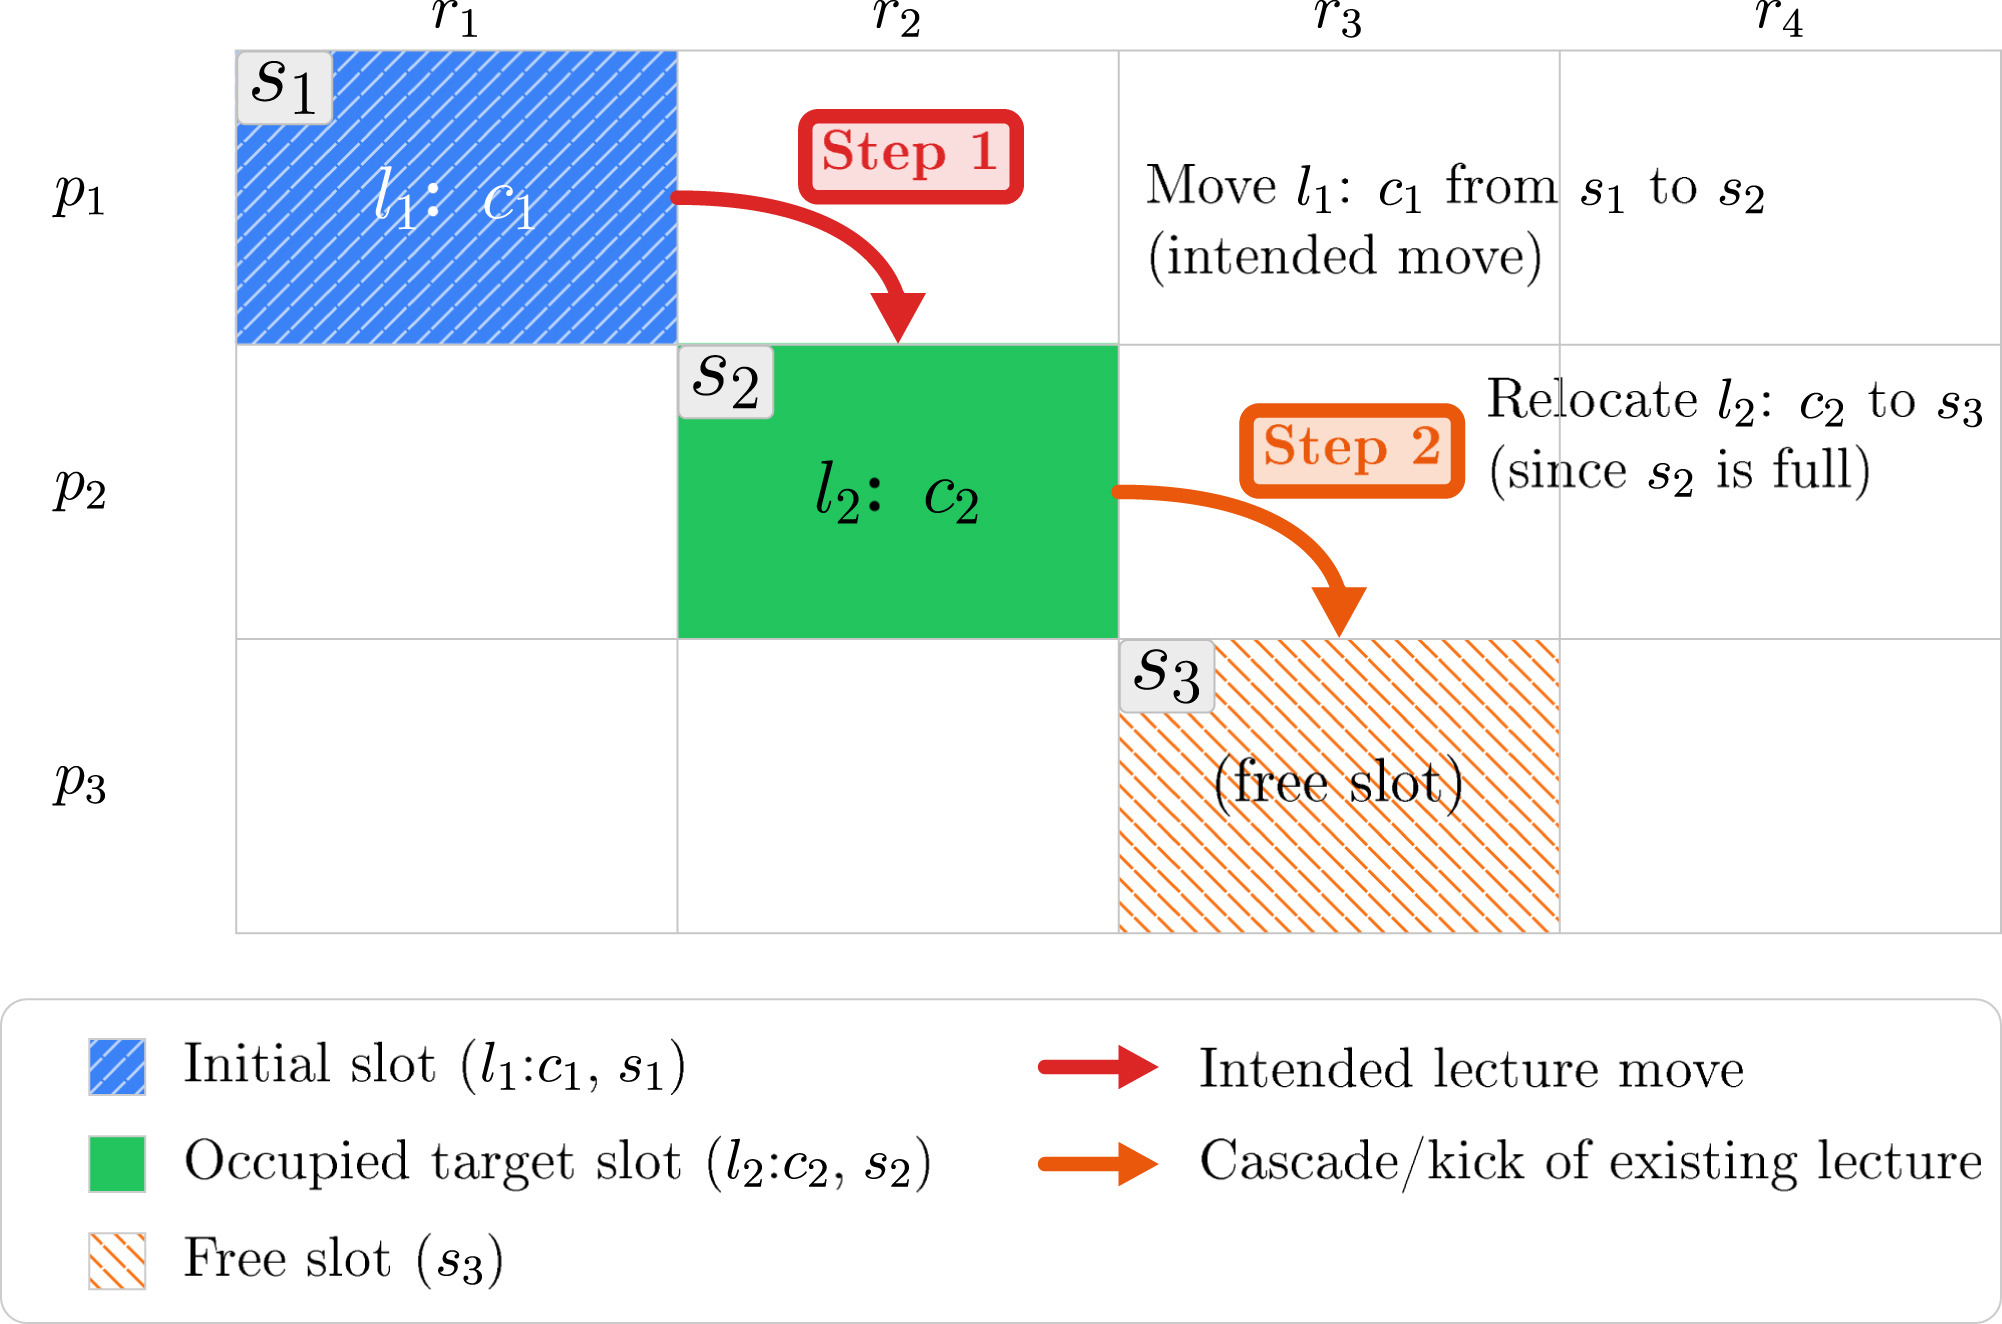
\includegraphics[width=0.98\columnwidth]{fig3.png}
\caption{Movimiento LectureKick. El símbolo li identifica una clase, ci su curso y si un hueco formado por periodo y aula. La clase l1 pasa de s1 a s2 y, si el destino está ocupado, l2 puede reubicarse en s3. Reproducido de la Fig. 1 de Ceschia et al. \cite{ref18}.}
\label{fig:lecturekick}
\end{figure}

Los destinos deben ser distintos, los periodos deben estar disponibles y las clases implicadas no pueden presentar conflictos. Cuando se utiliza s3, ese hueco debe permanecer libre. Estas condiciones hacen que la regla trabaje únicamente con horarios factibles.


La elección de movimientos tampoco es uniforme. El diseño estudiado por Ceschia et al. considera seis mecanismos de sesgo: días mínimos, cursos críticos vinculados a clases aisladas, capacidad, estabilidad de aula, preferencia por aulas adecuadas y frecuencia de intercambios. Tras el análisis de sensibilidad, no todos quedan como parámetros libres en la configuración final: el sesgo de capacidad se fija a 0 y la preferencia por aulas adecuadas se fija a 1, mientras que los restantes sesgos relevantes se afinan junto con los parámetros del enfriamiento simulado \cite{ref18}. La Fig.~\ref{fig:biases} resume los seis mecanismos considerados durante el diseño.


\begin{figure*}[!t]
\centering
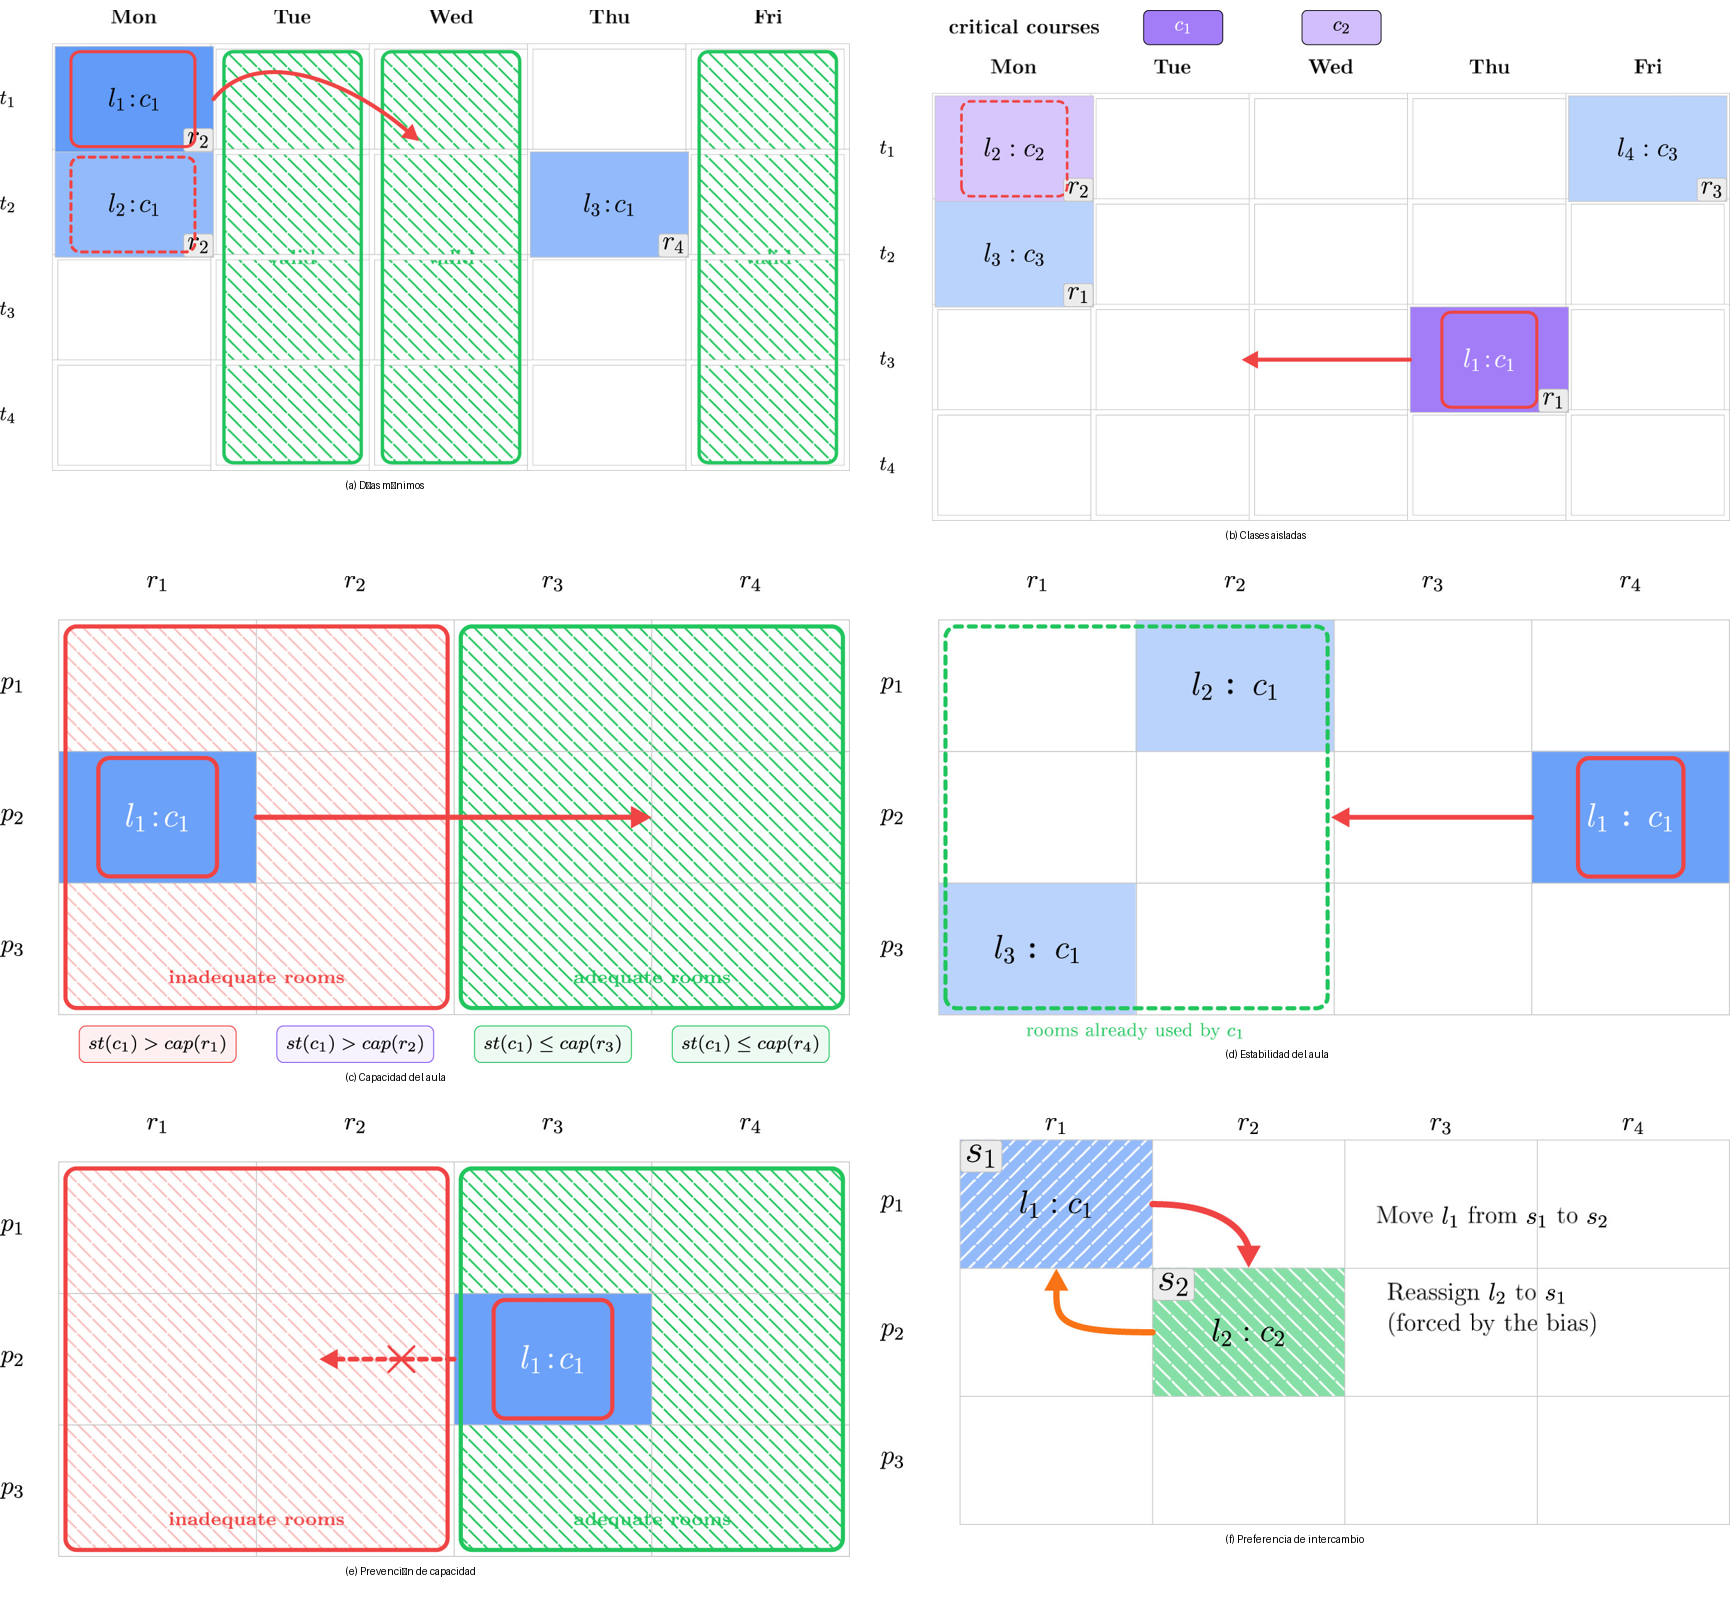
\includegraphics[width=0.92\textwidth]{fig4.png}
\caption{Ejemplos de los seis mecanismos de sesgo considerados en el diseño de LectureKick. En la configuración final, dos quedan fijados tras el análisis de sensibilidad y los restantes se combinan con los parámetros del enfriamiento simulado. Adaptado de la Fig. 2 de Ceschia et al. \cite{ref18}.}
\label{fig:biases}
\end{figure*}

Ceschia et al. emplearon irace para configurar automáticamente el método \cite{ref18}, \cite{ref19}. La afinación incluyó la temperatura inicial y final, la tasa de enfriamiento, el mecanismo de corte y las probabilidades de los sesgos que permanecieron activos tras el screening. Una vez seleccionada la configuración, sus valores se mantuvieron fijos durante la evaluación final. Esta distinción es importante porque la compilación ENHANCED del repositorio oficial conserva por compatibilidad opciones que ya no modifican el comportamiento final.


\section{Metodología de reproducción}

Se ejecutó el programa publicado por Ceschia et al. con la configuración utilizada en el artículo \cite{ref18}. El proceso comienza con Hill Climbing para obtener un horario factible y continúa con el enfriamiento simulado, que utiliza LectureKick para generar horarios vecinos.


\subsection{Diseño experimental}

Se seleccionaron las 19 instancias no redundantes de la formulación UD2 de ITC-2007. Se omitió comp11 porque su coste objetivo es nulo y comp15 porque equivale a comp03 bajo esta formulación. Cada instancia se ejecutó tres veces con semillas distintas, lo que dio lugar a 57 ejecuciones. El programa convirtió el límite virtual de 192 segundos en un presupuesto de búsqueda específico para cada instancia.


En cada ejecución, el programa construyó primero un horario y aplicó Hill Climbing hasta alcanzar una solución factible. Después utilizó enfriamiento simulado con LectureKick hasta agotar el presupuesto asignado. Al finalizar se verificaron el código de salida, el coste numérico y la ausencia de violaciones duras; además se conservaron el log y la solución de cada combinación instancia-semilla. Los scripts, results.csv, logs y soluciones de la campaña están disponibles en el repositorio del proyecto \cite{ref22}.


Por limitaciones computacionales, la reproducción emplea tres semillas por instancia frente a las 30 ejecuciones independientes del artículo y se ejecuta en un entorno diferente. En consecuencia, permite comprobar el procedimiento, la factibilidad y la estabilidad básica de la ejecución, pero no reproducir con la misma potencia estadística las medias y desviaciones publicadas. La Tabla~\ref{tab:entorno} resume las diferencias técnicas \cite{ref18}, \cite{ref20}.


\begin{table}[!t]
\caption{Diferencias técnicas entre el artículo de Ceschia et al. \cite{ref18} y la reproducción.}
\label{tab:entorno}
\centering
\footnotesize
\begin{tabular}{p{0.17\columnwidth} p{0.31\columnwidth} p{0.31\columnwidth}}
\toprule
\textbf{Aspecto} & \textbf{Artículo} & \textbf{Reproducción}\\
\midrule
CPU & Intel i7-7700 (4C/8T) & Intel i7-9700F (8C/8T)\\
SO & Ubuntu 24.04 & Windows 10 Pro\\
Compilador & G++ 13.3 & G++ 16.2 / UCRT64\\
\bottomrule
\end{tabular}
\end{table}

\section{Resultados}

\subsection{Validez de la campaña reproducida}

La campaña produjo 57/57 ejecuciones válidas mediante BHC-KSA, usando las semillas 0, 1 y 2, un límite virtual de 192 s, el commit 9cb3eb6 del solver y el commit b40b14c de EasyLocal++ 3. No se registró ninguna violación de restricciones duras. La configuración reproduce los parámetros finales de Ceschia et al. \cite{ref18}. El artículo se ejecutó en Ubuntu 24.04, GNU G++ 13.3 y un Intel Core i7-7700 a 3.60 GHz, utilizando un único núcleo virtual por ejecución; la reproducción se realizó en Windows 10, MSYS2 UCRT64, GNU G++ 16.2 e Intel i7-9700F. Por ello, los tiempos se utilizan como evidencia descriptiva y no como una réplica exacta del rendimiento temporal \cite{ref18}, \cite{ref20}.


\subsection{Comparación con el estudio de 2026 y con el estado del arte}

Para evitar confundir reproducibilidad con competitividad se emplean dos referencias distintas. Ceschia et al. \cite{ref18} resuelven cada instancia de validación mediante 30 ejecuciones y, en su Tabla 5, reportan media, desviación estándar, mínimo e iteraciones. Bajo el límite ITC-2007, su SA obtiene el mejor promedio en 7 de las 19 instancias y el mejor rango medio (1.79) entre los métodos comparados, aunque la prueba de Friedman no distingue globalmente a los métodos al nivel 0.05. Con solo tres semillas, la campaña de este trabajo no permite reproducir esas distribuciones ni repetir sus pruebas estadísticas; por ello, la comparación con \cite{ref18} se interpreta como reproducción funcional del protocolo. De forma separada, la Tabla~\ref{tab:entorno}I utiliza los mejores valores conocidos/upper bounds compilados en \cite{ref2} para medir distancia al estado del arte, y no atribuye esos valores al algoritmo de 2026.


\begin{table*}[!t]
\caption{Competitividad de la reproducción frente a los mejores valores conocidos (UB/best-known) compilados en \cite{ref2}. Un gap positivo indica un coste mayor que el best-known.}
\label{tab:results}
\centering
\footnotesize
\setlength{\tabcolsep}{5pt}
\begin{tabular}{lrrrrr}
\toprule
\textbf{Inst.} & \textbf{Best-known} & \textbf{Mejor} & \textbf{Media} & \textbf{Gap mejor} & \textbf{$t$ medio (s)}\\
\midrule

comp01 & 5 & 5 & 5.00 & 0.0\% & 335.2\\

comp02 & 24 & 42 & 44.00 & 75.0\% & 338.3\\

comp03 & 64 & 76 & 76.00 & 18.8\% & 278.1\\

comp04 & 35 & 37 & 38.33 & 5.7\% & 280.5\\

comp05 & 284 & 300 & 308.33 & 5.6\% & 376.5\\

comp06 & 27 & 36 & 38.67 & 33.3\% & 326.1\\

comp07 & 6 & 12 & 13.33 & 100.0\% & 335.1\\

comp08 & 37 & 39 & 39.67 & 5.4\% & 287.7\\

comp09 & 96 & 101 & 101.00 & 5.2\% & 295.5\\

comp10 & 4 & 10 & 12.00 & 150.0\% & 322.1\\

comp12 & 294 & 318 & 322.67 & 8.2\% & 294.2\\

comp13 & 59 & 59 & 64.00 & 0.0\% & 276.3\\

comp14 & 51 & 53 & 53.00 & 3.9\% & 265.8\\

comp16 & 18 & 29 & 31.33 & 61.1\% & 283.8\\

comp17 & 56 & 68 & 71.33 & 21.4\% & 292.2\\

comp18 & 61 & 71 & 71.33 & 16.4\% & 236.8\\

comp19 & 57 & 59 & 60.00 & 3.5\% & 282.9\\

comp20 & 4 & 18 & 19.00 & 350.0\% & 350.0\\

comp21 & 74 & 86 & 94.00 & 16.2\% & 289.7\\

\bottomrule
\end{tabular}
\end{table*}

El mejor resultado reproducido igualó el best-known de \cite{ref2} en 2 de 19 instancias: comp01 (5) y comp13 (59). En las otras 17 instancias el mejor coste fue superior. El gap porcentual mediano fue 16.2\%; la media fue 46.3\%, valor muy influido por instancias con referencias pequeñas como comp10 y comp20. La media de los mejores costes reproducidos fue 74.68 frente a 66.11 para los best-known. Estas cifras describen competitividad frente al estado del arte y no equivalencia con las 30 ejecuciones del algoritmo de 2026. El tiempo medio reportado por el solver fue 302.5 s por ejecución, pero no es directamente comparable con el tiempo de referencia porque cambia el entorno y el límite virtual se transforma en un número de iteraciones específico por instancia \cite{ref18}.


\begin{figure}[!t]
\centering
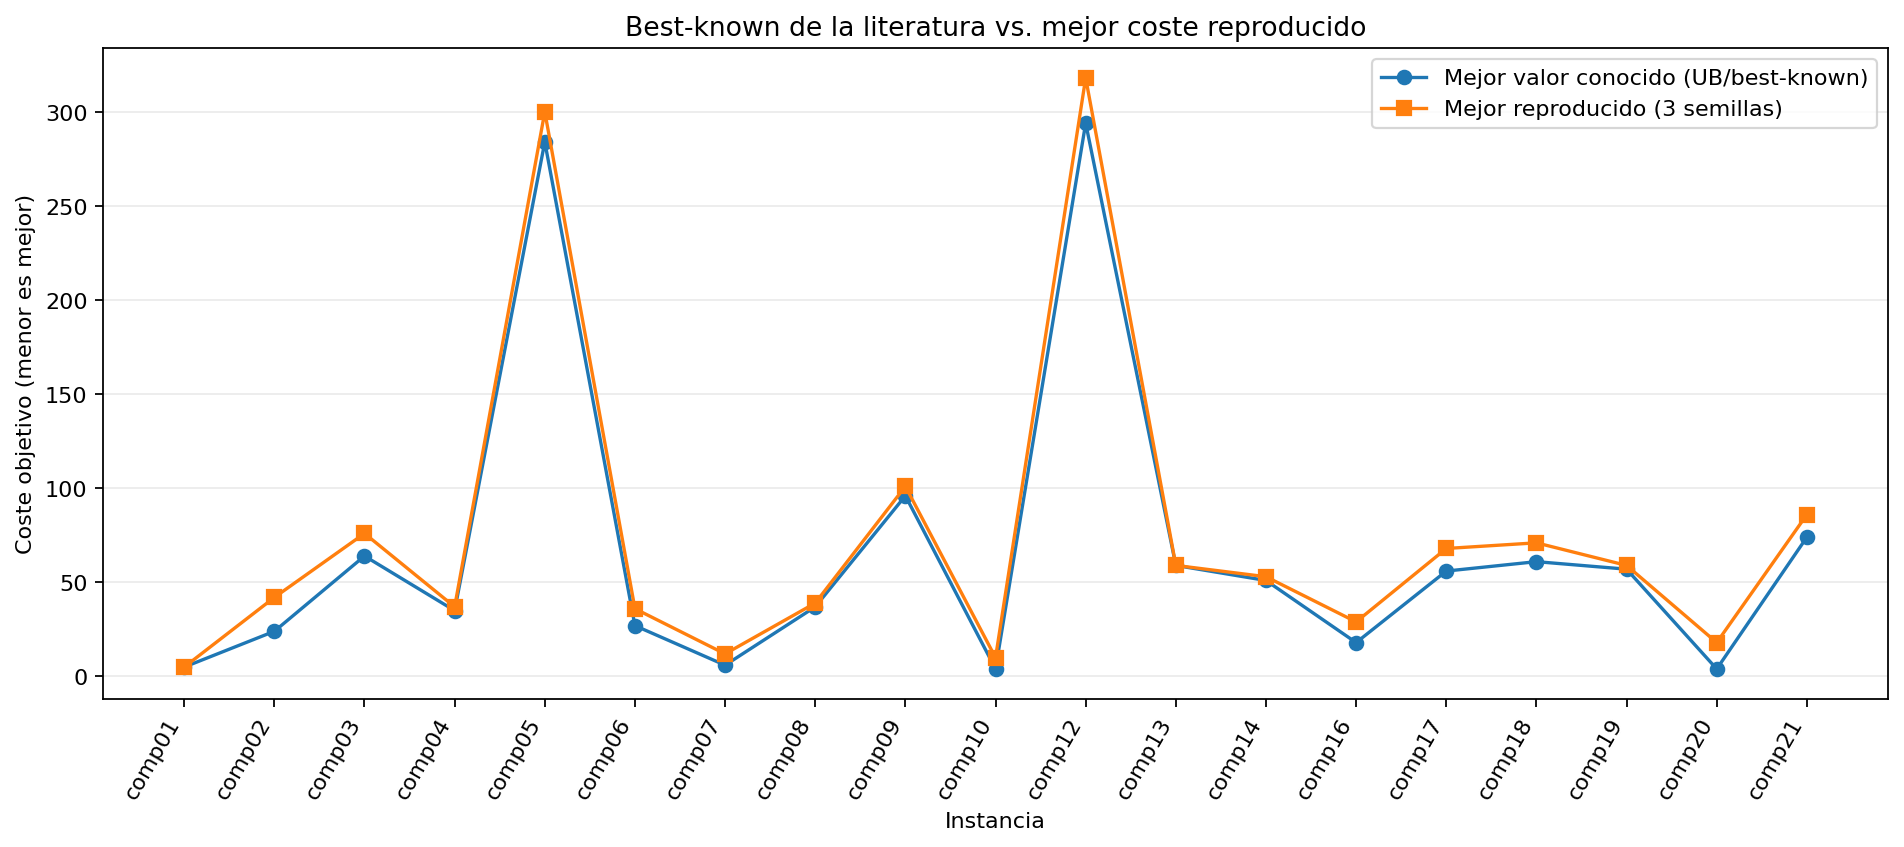
\includegraphics[width=\columnwidth]{fig5.png}
\caption{Mejor coste reproducido frente al mejor valor conocido (UB/best-known) de \cite{ref2} para las 19 instancias no redundantes.}
\label{fig:costs}
\end{figure}

\begin{figure}[!t]
\centering
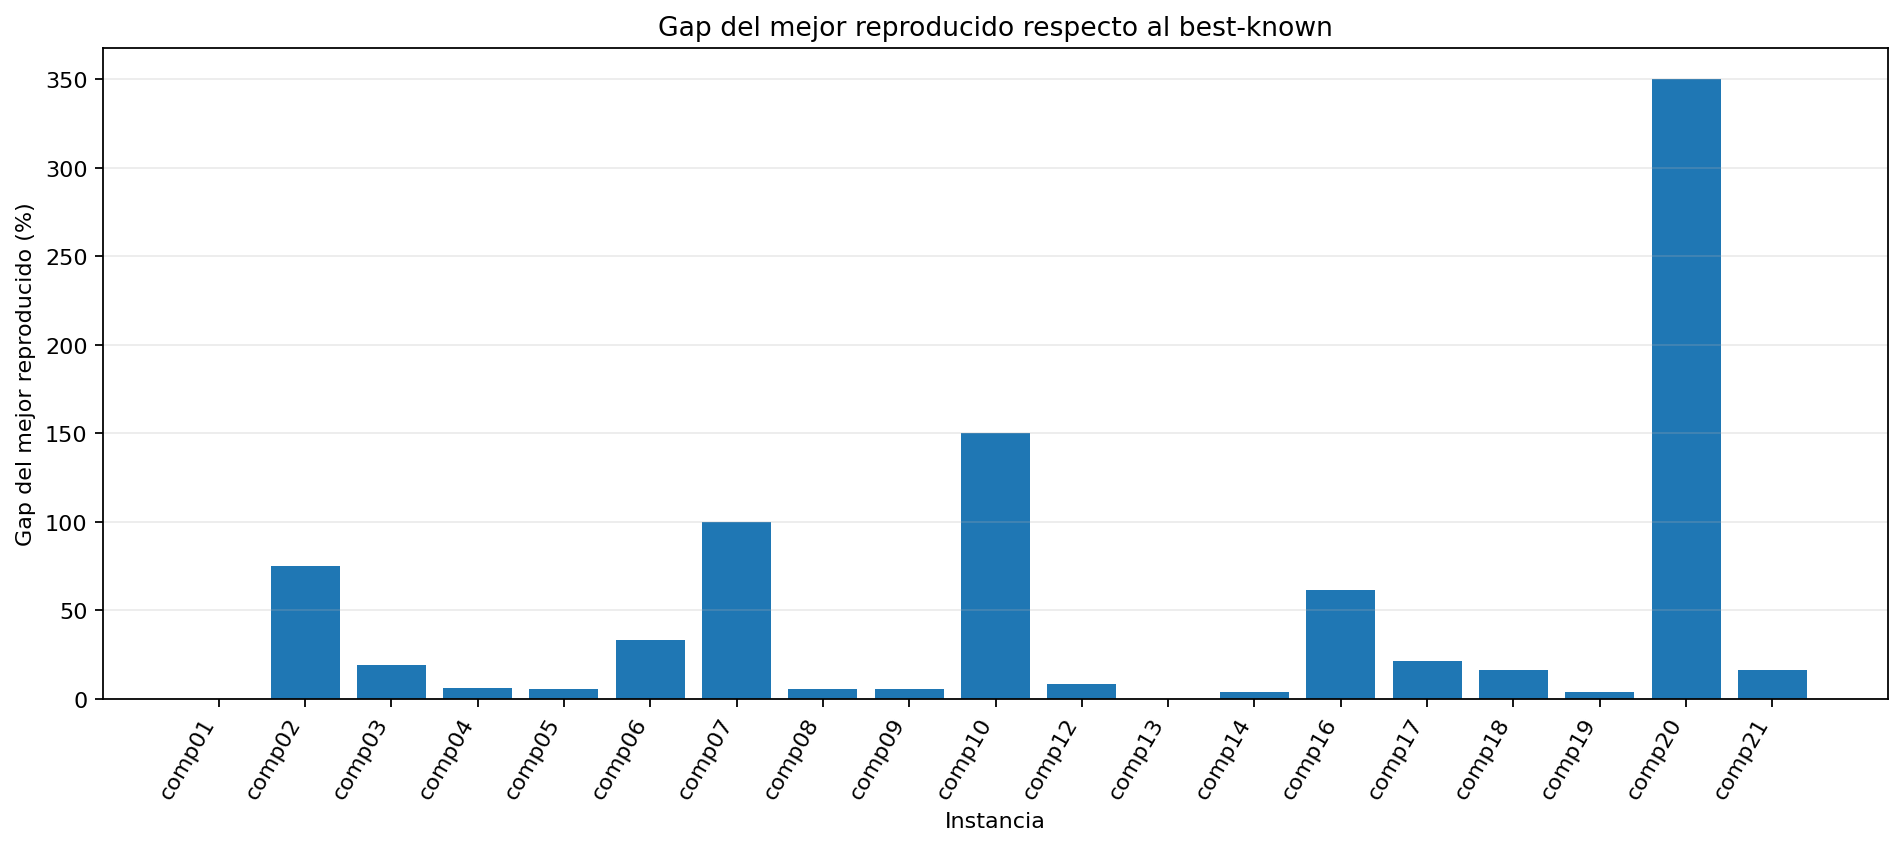
\includegraphics[width=\columnwidth]{fig6.png}
\caption{Gap del mejor coste reproducido respecto al mejor valor conocido de \cite{ref2} por instancia.}
\label{fig:gap}
\end{figure}

\subsection{Resultados de la revisión cuantitativa}\label{subsec:reviewquant}

La matriz de extracción contiene 25 estudios primarios de 2015--2026: 21 corresponden al núcleo CB-CTT y 4 a extensiones explícitas. En este corpus, los métodos exactos, matemáticos y declarativos constituyen la mayor familia individual (28\%), mientras que búsqueda local, métodos evolutivos y aprendizaje automático/selección/configuración representan 16\% cada uno. Dieciséis estudios (64\%) utilizan explícitamente ITC-2007. Veinte (80\%) usan datos públicos o mayoritariamente públicos, pero solo en dos (8\%) se verificó código público junto con una configuración suficientemente detallada para clasificarlos con reproducibilidad alta. La comparación entre estas cifras muestra una diferencia clara entre disponibilidad del benchmark y disponibilidad del experimento ejecutable.


\begin{figure}[!t]
\centering
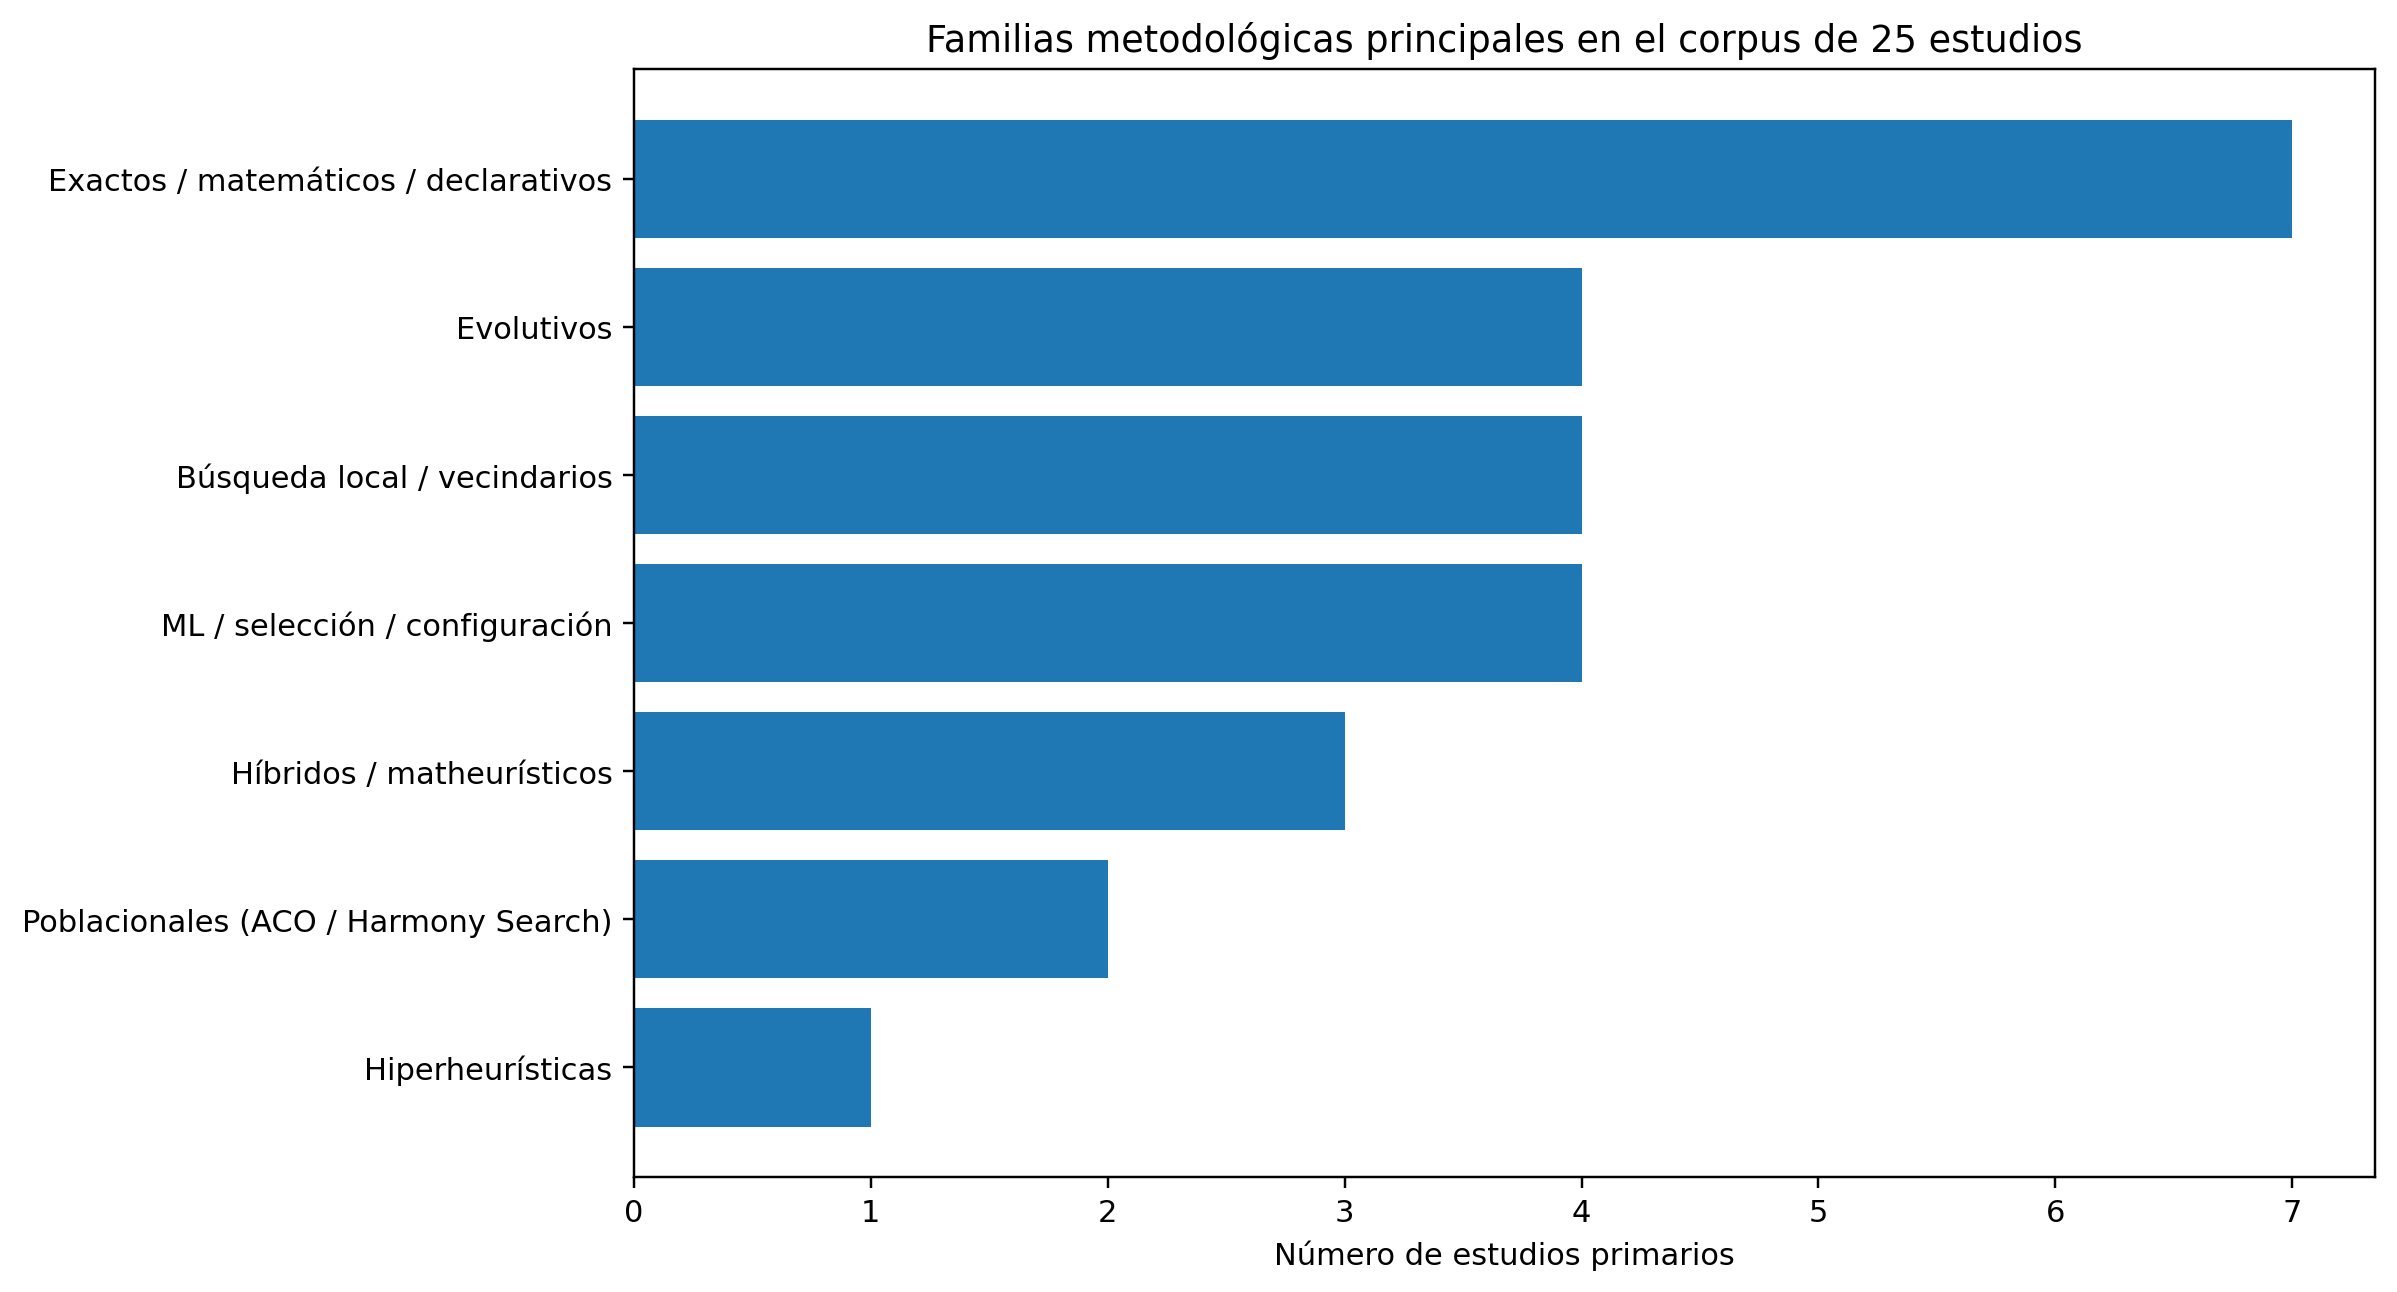
\includegraphics[width=\columnwidth]{fig7.png}
\caption{Distribución de las familias metodológicas principales en los 25 estudios primarios.}
\label{fig:families}
\end{figure}

\begin{figure*}[!t]
\centering
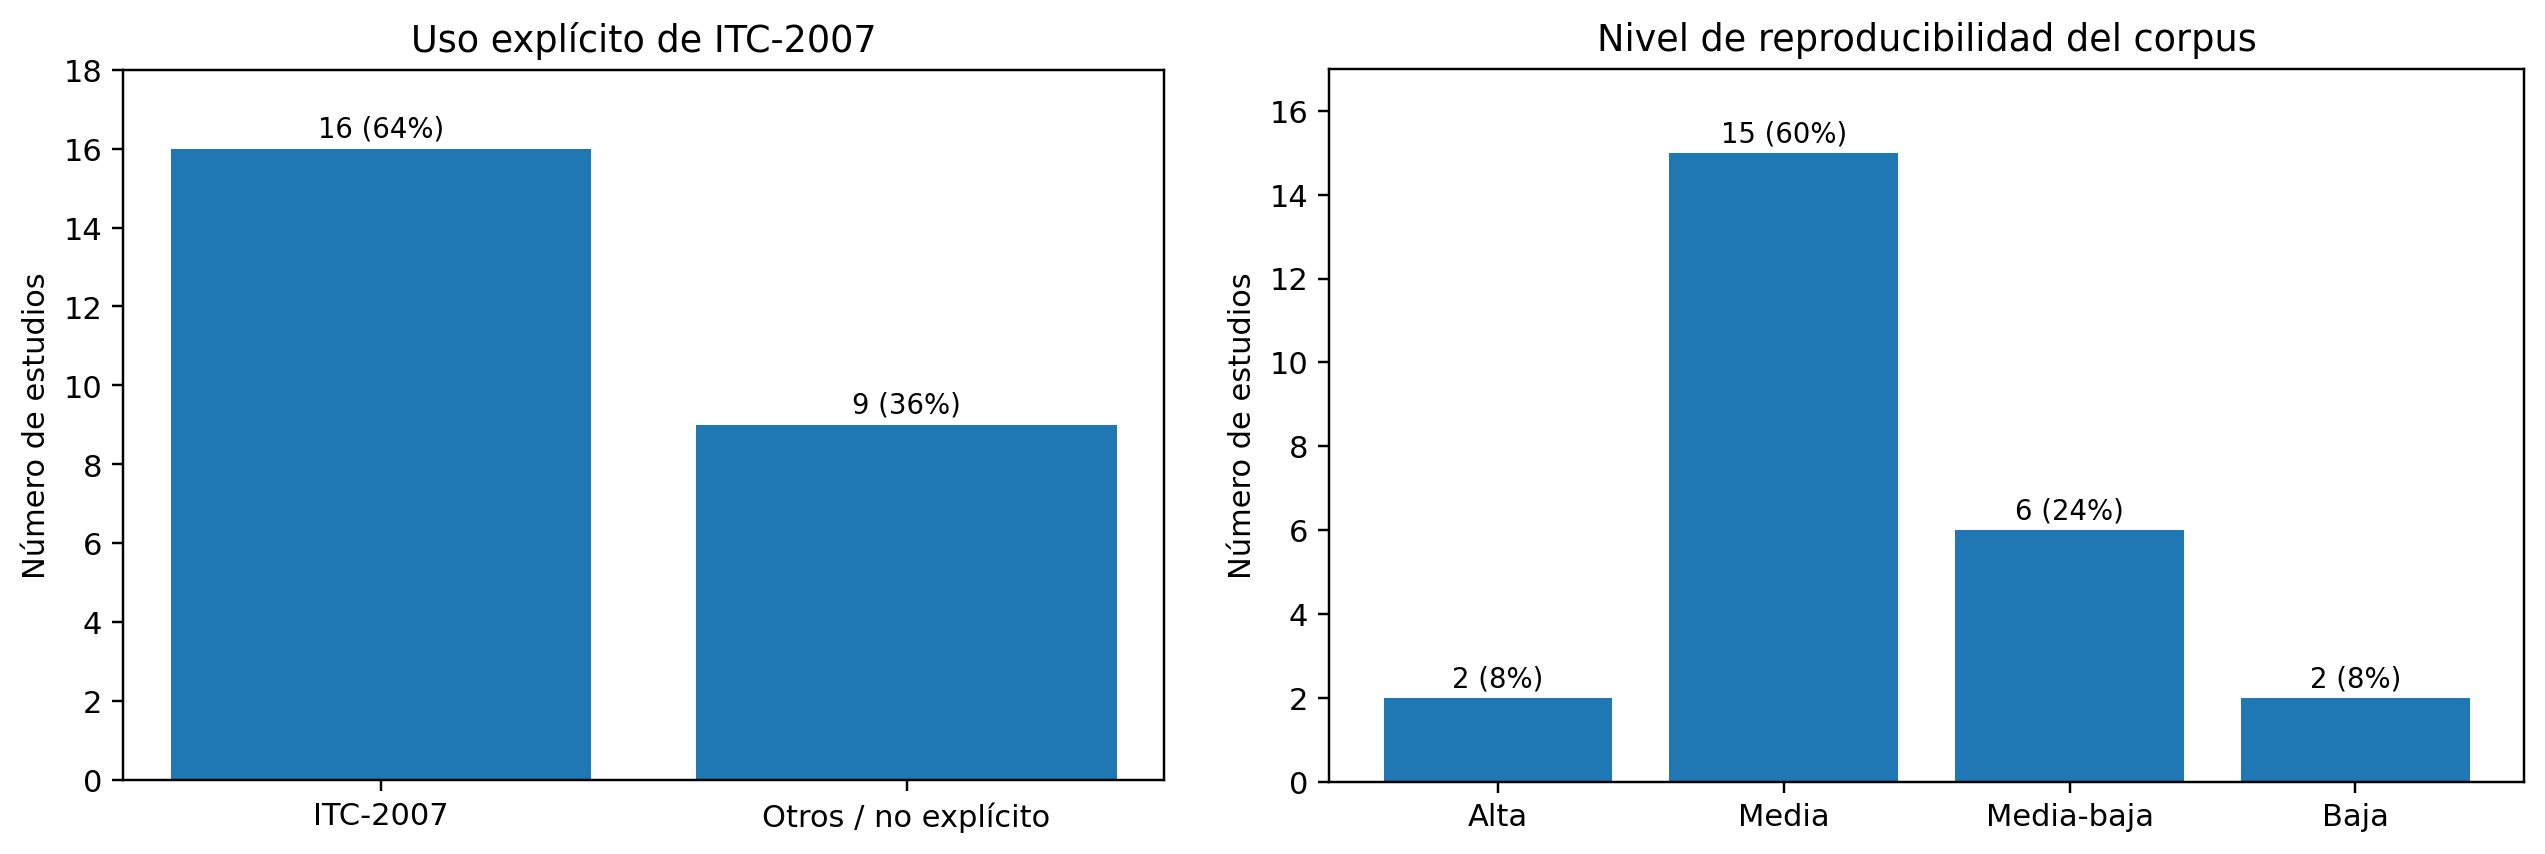
\includegraphics[width=0.88\textwidth]{fig8.png}
\caption{Uso explícito de ITC-2007 y niveles de reproducibilidad en el corpus de 25 estudios primarios.}
\label{fig:repro}
\end{figure*}

\section{Discusión y amenazas a la validez}

La reproducción confirma la factibilidad técnica del artefacto de Ceschia et al. \cite{ref18}: el código compila, las 57 ejecuciones terminan correctamente y las soluciones respetan todas las restricciones duras. Sin embargo, no reproduce la distribución estadística reportada por el artículo, que emplea 30 ejecuciones independientes por instancia. Tres semillas permiten verificar el procedimiento y observar variabilidad básica, pero no afirmar equivalencia estadística entre medias o desviaciones. La distancia frente a los best-known de la Tabla~\ref{tab:entorno}I tampoco constituye un fallo del artefacto: esos valores agregan resultados de distintos métodos y presupuestos computacionales \cite{ref2}, mientras que la campaña ejecutada aquí usa un único protocolo y solo tres semillas.


La principal amenaza a la validez interna procede del cambio de plataforma y del reducido número de repeticiones. Aunque BHC-KSA convierte el límite virtual en un presupuesto de iteraciones para reducir la dependencia del hardware, el tiempo medido continúa afectado por sistema operativo, compilador, CPU y sobrecarga de E/S. En consecuencia, la comparación debe centrarse en factibilidad y calidad de las soluciones, no en igualdad de segundos. Para una réplica estadística del estudio de 2026 sería necesario ejecutar 30 repeticiones por instancia y reproducir las mismas pruebas estadísticas de \cite{ref18}.


Respecto a la validez externa, ITC-2007 sigue siendo útil porque ofrece una función objetivo y restricciones estandarizadas y aparece explícitamente en el 64\% del corpus analizado. No obstante, ITC-2019 incorpora student sectioning, estructuras de clases y restricciones institucionales más ricas \cite{ref5}. Por ello, un algoritmo competitivo en UD2 no puede considerarse automáticamente adecuado para todas las configuraciones universitarias actuales. Los trabajos recientes amplían la evaluación con otras familias reales, instancias sintéticas y enfoques híbridos o adaptativos \cite{ref17}, \cite{ref18}, \cite{ref21}.


\section{Conclusiones}

En el corpus analizado, CB-CTT muestra una evolución hacia la combinación de optimización exacta, metaheurísticas, hibridación y mecanismos de adaptación. El aprendizaje automático aparece principalmente como apoyo para selección, caracterización y configuración de algoritmos, no como sustituto directo del optimizador \cite{ref17}, \cite{ref4}. ITC-2007 continúa siendo la referencia común más frecuente del corpus, pero se complementa con conjuntos de datos más diversos para estudiar generalización y realismo.


Experimentalmente, se reprodujo de extremo a extremo el artefacto BHC-KSA/LectureKick sobre 19 instancias y tres semillas, obteniéndose 57 soluciones factibles sin violaciones duras. La reproducción funcional del protocolo de \cite{ref18} debe distinguirse de la comparación de competitividad: el mejor coste igualó el best-known de la literatura en comp01 y comp13, mientras que en las demás instancias permaneció por encima. Dado que la campaña utiliza solo tres repeticiones y un entorno distinto, no constituye una réplica estadística completa del artículo de 2026. El mismo contraste aparece en la revisión: en el corpus analizado los benchmarks son mayoritariamente públicos, pero el código y la configuración completa son mucho menos frecuentes.


\balance

\begin{thebibliography}{22}

\bibitem{ref1} L. Di Gaspero, B. McCollum y A. Schaerf, The Second International Timetabling Competition (ITC-2007): Curriculum-Based Course Timetabling (Track 3), 2007.

\bibitem{ref2} S. Ceschia, L. Di Gaspero y A. Schaerf, "Educational timetabling: Problems, benchmarks, and state-of-the-art results," European Journal of Operational Research, vol. 308, no. 1, pp. 1-18, 2023. doi:10.1016/j.ejor.2022.07.011.

\bibitem{ref3} A. Bettinelli, V. Cacchiani, R. Roberti y P. Toth, "An overview of curriculum-based course timetabling," TOP, vol. 23, pp. 313-349, 2015. doi:10.1007/s11750-015-0366-z.

\bibitem{ref4} X. Gu, M. Krish, S. Sohail, S. Thakur, F. Sabrina y Z. Fan, "From Integer Programming to Machine Learning: A Technical Review on Solving University Timetabling Problems," Computation, vol. 13, no. 1, 10, 2025. doi:10.3390/computation13010010.

\bibitem{ref5} T. Müller, H. Rudová y Z. Müllerová, "Real-world university course timetabling at the International Timetabling Competition 2019," Journal of Scheduling, vol. 28, pp. 247-267, 2025. doi:10.1007/s10951-023-00801-w.

\bibitem{ref6} N.-C. F. Bagger, S. Kristiansen, M. Sørensen y T. R. Stidsen, "Flow formulations for curriculum-based course timetabling," Annals of Operations Research, vol. 280, pp. 121-150, 2019. doi:10.1007/s10479-018-3096-4.

\bibitem{ref7} N.-C. F. Bagger, M. Sørensen y T. R. Stidsen, "Dantzig-Wolfe decomposition of the daily course pattern formulation for curriculum-based course timetabling," European Journal of Operational Research, vol. 272, no. 2, pp. 430-446, 2019. doi:10.1016/j.ejor.2018.06.042.

\bibitem{ref8} R. Asín Achá y R. Nieuwenhuis, "Curriculum-based course timetabling with SAT and MaxSAT," Annals of Operations Research, vol. 218, pp. 71-91, 2014. doi:10.1007/s10479-012-1081-x.

\bibitem{ref9} M. Banbara et al., "teaspoon: solving the curriculum-based course timetabling problems with answer set programming," Annals of Operations Research, vol. 275, pp. 3-37, 2019. doi:10.1007/s10479-018-2757-7.

\bibitem{ref10} T. Müller, "ITC2007 solver description: A hybrid approach," Annals of Operations Research, vol. 172, no. 1, pp. 429-446, 2009. doi:10.1007/s10479-009-0644-y.

\bibitem{ref11} C. Ababei, "Speeding up FPGA placement via partitioning and multithreading," International Journal of Reconfigurable Computing, vol. 2009, pp. 1-9, 2009.

\bibitem{ref12} R. Bellio, S. Ceschia, L. Di Gaspero, A. Schaerf y T. Urli, "Feature-based tuning of simulated annealing applied to the curriculum-based course timetabling problem," Computers \& Operations Research, vol. 65, pp. 83-92, 2016. doi:10.1016/j.cor.2015.07.002.

\bibitem{ref13} T. Song et al., "Competition-guided multi-neighborhood local search algorithm for the university course timetabling problem," Applied Soft Computing, vol. 110, 107624, 2021. doi:10.1016/j.asoc.2021.107624.

\bibitem{ref14} S. Abdullah, H. Turabieh, B. McCollum y P. McMullan, "A hybrid metaheuristic approach to the university course timetabling problem," Journal of Heuristics, vol. 18, pp. 1-23, 2012. doi:10.1007/s10732-010-9154-y.

\bibitem{ref15} S. Abdipoor, R. Yaakob, S. L. Goh y S. Abdullah, "Meta-heuristic approaches for the university course timetabling problem," Intelligent Systems with Applications, vol. 19, 200253, 2023. doi:10.1016/j.iswa.2023.200253.

\bibitem{ref16} A. Kiefer, R. F. Hartl y A. Schnell, "Adaptive large neighborhood search for the curriculum-based course timetabling problem," Annals of Operations Research, vol. 252, no. 2, pp. 255-282, 2017. doi:10.1007/s10479-016-2151-2.

\bibitem{ref17} A. De Coster, N. Musliu, A. Schaerf, J. Schoisswohl y K. Smith-Miles, "Algorithm selection and instance space analysis for curriculum-based course timetabling," Journal of Scheduling, vol. 25, no. 1, pp. 35-58, 2022. doi:10.1007/s10951-021-00701-x.

\bibitem{ref18} S. Ceschia, F. Da Ros, L. Di Gaspero y A. Schaerf, "Revisiting local search for Curriculum-Based Course Timetabling," Computers \& Operations Research, vol. 195, 107621, 2026. doi:10.1016/j.cor.2026.107621.

\bibitem{ref19} M. López-Ibáñez, J. Dubois-Lacoste, L. Pérez Cáceres, T. Stützle y M. Birattari, "The irace package: Iterated Racing for Automatic Algorithm Configuration," Operations Research Perspectives, vol. 3, pp. 43-58, 2016. doi:10.1016/j.orp.2016.09.002.

\bibitem{ref20} L. M. Weber et al., "Essential guidelines for computational method benchmarking," Genome Biology, vol. 20, art. 125, 2019. doi:10.1186/s13059-019-1738-8.

\bibitem{ref21} T. M. Nguyen, "Adaptive Penalty-Guided VND with CP-SAT for Curriculum-Based Course Timetabling," in Proc. 18th Int. Conf. on Agents and Artificial Intelligence (ICAART), vol. 4, SciTePress, pp. 3398-3405, 2026. doi:10.5220/0014437700004052.

\bibitem{ref22} A. Moris Lara, J. Martin La Peña y J. M. Villacorta Arteaga, ``uctp-optimization-ai-review: materiales y artefactos de la revisión y reproducción de CB-CTT,' GitHub, 2026. Disponible: \url{https://github.com/alejandromorislara/uctp-optimization-ai-review}

\end{thebibliography}

\end{document}
